\section{Résultats}

\paragraph{Étalonnage des transformateurs}
Les cycles à vide des transformateurs permettent de trouver \(\alpha\) tel que \(V_f = \alpha V_i\). Une régression linéaire sur le cycle du transformateur PHYWE à la \autoref{fig:phywe_vide} permet d'obtenir \(V_f = (truc) V_i\). Une régression linéaire sur le cycle du transformateur cylindrique à la \autoref{fig:cylindre_vide} donne \(V_f = (truc) V_i\). Le transformateur cylindrique ne présente pas d'hystérèse à vide, alors que le transformateur PHYWE possède une légère hystérèse, mais l'écart entre les courbes en montée et en descente est très faible, et les courbes restent linéaires sur une majeure partie du graphe.

\begin{figure}[h]
    \centering
    \begin{subfigure}{0.5\linewidth}
        \centering
        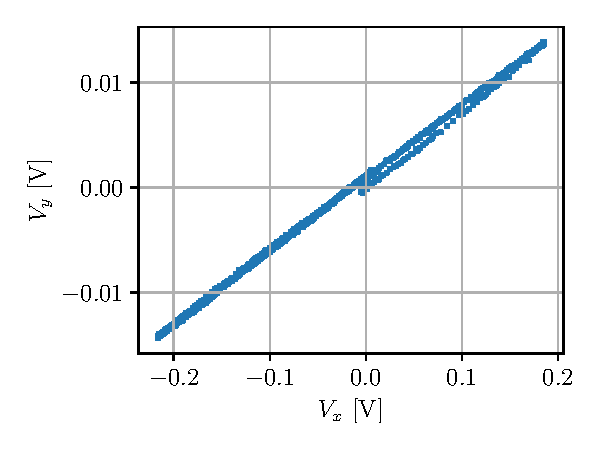
\includegraphics[width=\linewidth]{figures/G1-phywe-vide.pdf}
        \caption{}
        \label{fig:phywe_vide}
    \end{subfigure}%
    \begin{subfigure}{0.5\linewidth}
        \centering
        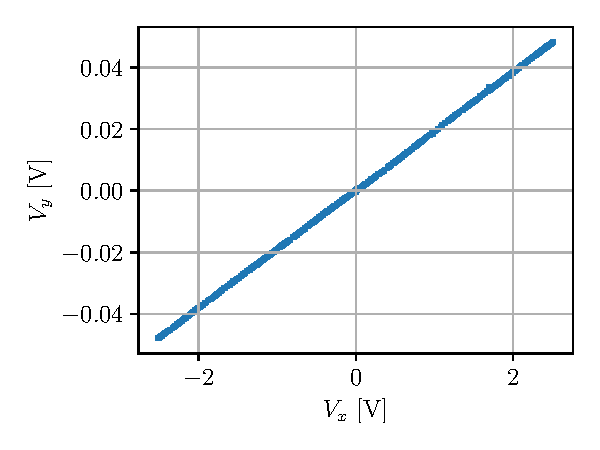
\includegraphics[width=\linewidth]{figures/G1-cylindre-vide.pdf}
        \caption{}
        \label{fig:cylindre_vide}
    \end{subfigure}
    \caption{Cycles à vide sur les transformateur (a) \textit{PhyWe} (b) cylindrique}
\end{figure}

\paragraph{Propriétés des matériaux}
Les différents matériaux mesurés ont présenté des comportements magnétiques différents. Leur classification a pu être déterminée en connaissant leur valeur de \(\mu_r\) qui a été obtenue par l'équation \autoref{eq:mu_r} à l'aide des régressions linéaires sur les transformateurs à vide et sur les parties linéaires des graphiques des différents matériaux. Pour les matériaux présentant un comportement non linéaire TODO: comme illustré dans la figure. Cette classification avec les valeurs des \(\mu_r\) est présentée dans le \autoref{tab:mu_r}.

\begin{table}[h]
    \centering
    \begin{tabulary}{\linewidth}{c c c c c c c}
        \toprule
        & Acier doux & Aluminium & Cuivre & Acier-Ag-Cr & Nickel-200 & Monel-400 \\
        \midrule
        \(\mu_r\) pour PHYWE & \(1.16 \pm 0.04\) & \(1.08 \pm 0.01\) & \(1.08 \pm 0.01\) & - & - & - \\
        \(\mu_r\) pour Cylindre & \(2.48 \pm 0.08\) & \(0.99 \pm 0.01\) & \(0.98 \pm 0.01\) & \(2.1 \pm 0.1\) & \(1.11 \pm 0.01\) & \(1.09 \pm 0.01\) \\
        Magnétisme & Ferro- & - & - & Ferro- & Para- & Para- \\
        \bottomrule
    \end{tabulary}
    \caption{Valeurs de \(\mu_r\) pour différents échantillons dans chaque transformateur et leurs types de magnétisme (Ferro-, Para- et Dia- magnétisme)}
    \label{tab:mu_r}
\end{table}


\begin{minipage}{\linewidth}
    \begin{wrapfigure}{R}{0.5\linewidth}
        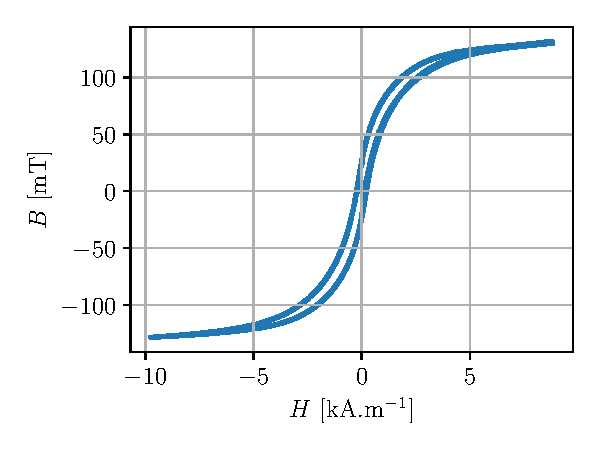
\includegraphics[width=\linewidth]{figures/G1-phywe-avec-bloc_chang.pdf}
        \caption{Cycle d'hystérèse du bloc PHYWE}
        \label{fig:calibr_phywe}
    \end{wrapfigure}

    \paragraph{Callibration des axes}
    A partir des équations \autoref{eq:calibr_H} et \autoref{eq:calibr_B} il est possible de calculer les constantes pour pouvoir changer de variables et obtenir une induction magnétique en fonction d'un champ. En prenant pour le transformateur PHYWE \(L = 6.4 \pm 0.1\) \si{\centi \meter} et \(N = 600\) le nombre de spire du primaire, les coefficients obtenus lorsque le bloc PHYWE est utilisé sont: \(H = (4.6\pm0.1)\times10^3 V_i\) et \(B = (8.3\pm0.2)\times10^{-2} V_f\). La figure avec les axes calibrés est visible en \autoref{fig:calibr_phywe}.
    Ces nouveaux graphiques permettent de mieux visualiser le système physique et les caractéristiques principales de son hystérèse à savoir les valeurs des \(H_c\), \(H_S\), \(B_r\) et \(B_S\). Pour le bloc PHYWE la valeur du champ coercitif après saturation est donc très proche de 0 \si{\kilo\ampere\per\meter}. Les valeurs de saturation  du champ magnétique et de l'induction respectivement peuvent être lues aux alentour de 10 \si{\kilo\ampere\per\meter} et 200 \si{\milli\tesla}.
\end{minipage}



\paragraph{Trucs supplémentaires}
Titre à revoir, en gros les différents cycle d'hystérèse, les différentes épaisseurs, les plaques amagnétiques...


\begin{minipage}{\linewidth}
    \paragraph{Échantillons empilés}
    La \autoref{fig:combo} est obtenue en empillant deux échantillons du même matériau. Les épaisseurs des échantillons sont dans le \autoref{tab:thiccness} en \autoref{sec:resultats_bonus}. La réponse au champ magnétique varie en fonction de l'épaisseur du matériau.

    \begin{wrapfigure}{R}{0.6\linewidth}
        \centering
        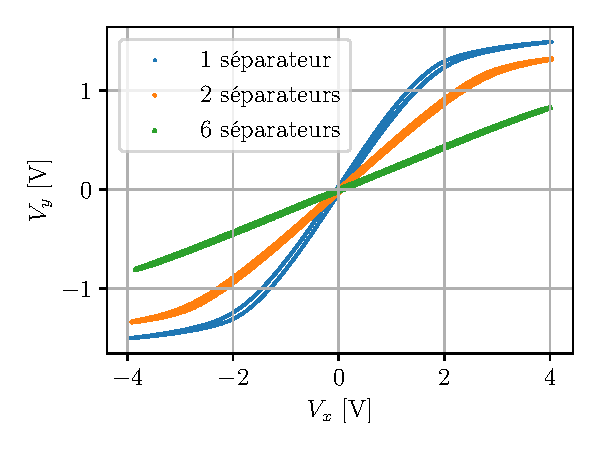
\includegraphics[width=\linewidth]{figures/separateurs_amagnetique.pdf}
        \caption{Réponse du bloc PHYWE après insertion de 1, 2 et 6 séparateurs amagnétiques}
        \label{fig:amagnetique}
    \end{wrapfigure}

    \paragraph{Plaques amagnétiques}
    L'insertion de plaques amagnetique entre le transformateur et le bloc PHYWE change aussi la réponse du bloc, comme le montre la \autoref{fig:amagnetique}. Un nombre plus grand, correspondant à une plus grande épaisseur, de plaques amagnétiques diminue et même élimine le cycle d'hystérèse du bloc, qui répond alors linéairement au changement de champ magnétique.

    \paragraph{Orientation du bloc PHYWE}
    belle bite shinji
\end{minipage}
    
